\documentclass[10pt,a4paper]{article}
\usepackage[margin=1.65 cm,top=1.4 cm,bottom=1.5 cm]{geometry}
\usepackage[T1]{fontenc}
\usepackage[utf8]{inputenc}
\usepackage{lmodern,microtype,booktabs,tabularx,array,amsmath,graphicx,xcolor,hyperref,enumitem,fancyhdr}
\definecolor{navy}{HTML}{183B56}\definecolor{teal}{HTML}{187F80}
\hypersetup{colorlinks=true,urlcolor=teal,linkcolor=navy,pdftitle={Thesis Progress Update: Routing Cost and Training-Energy Payback},pdfauthor={Eren Olmez}}
\setlength{\parindent}{0 pt}\setlength{\parskip}{4 pt}\setlength{\emergencystretch}{2 em}
\renewcommand{\arraystretch}{1.12}
\setlist[itemize]{leftmargin=1.2 em,itemsep=1 pt,topsep=2 pt}
\pagestyle{fancy}\fancyhf{}\fancyhead[L]{\small\color{navy}Energy-efficient input-based model routing}
\fancyhead[R]{\small 29 October 2026}\fancyfoot[C]{\small\thepage}\setlength{\headheight}{13 pt}
\newcommand{\heading}[1]{\section*{\color{navy}#1}}
\newcommand{\smallcap}[1]{{\footnotesize\color{navy}#1}\par}
\begin{document}
\begin{center}
{\Large\bfseries\color{navy}Thesis Progress Update}\\[3 pt]
{Eren Olmez}\\{29 October 2026}
\end{center}\vspace{-8 pt}
\heading{1. Meeting questions and results across batch sizes}
The meeting requested batch-level accuracy, latency and energy statistics including batch 1, clearer plots, and the number of deployment inferences needed to recover router-training energy. This update joins the saved 13 October correctness results and 20 October controls with the new batch 1 investigations. No larger-batch experiments were rerun.

\textbf{What is being routed?} The router is a small predictor that chooses which classifier will process an input. Our correctness TinyCNN predicts each candidate's probability of success; a calibrated cost rule selects one classifier, which predicts the CIFAR-100 class. For a batch, probabilities are averaged to select one model for all its images. Fitting used 3,000 images and calibration 2,000; evaluation uses all 10,000 balanced test images (100 per class).

\textbf{Two routing studies and separate probes.} Study A changes the \emph{router architecture}; Study B changes \emph{how the same TinyCNN system loads and executes classifiers}. Separate engineering probes test ideas not adopted in those full routing runs. These are not one system containing every optimization.

\textbf{Baseline and pass.} Eligible static means one fixed classifier selected on calibration data to meet the accuracy allowance, without routing. Savings compare fresh measurements in the same execution mode (eager or Graph). An accuracy pass alone does not imply an efficiency win.

\textbf{Comparison rule.} Policies below were calibrated for latency at 1 percentage point (pp), seeds 42/45/48. Tables now assess the \emph{same frozen policies} at both 1 pp ($\geq 84.80\%$ accuracy) and 2 pp ($\geq 83.80\%$), versus R101 FP32's 85.80\%. No 2 pp recalibration or new run is claimed. Historical costs are five-repeat medians; batch 1 has one sweep per seed. A looser pass is not itself a speed/energy improvement.
\begin{center}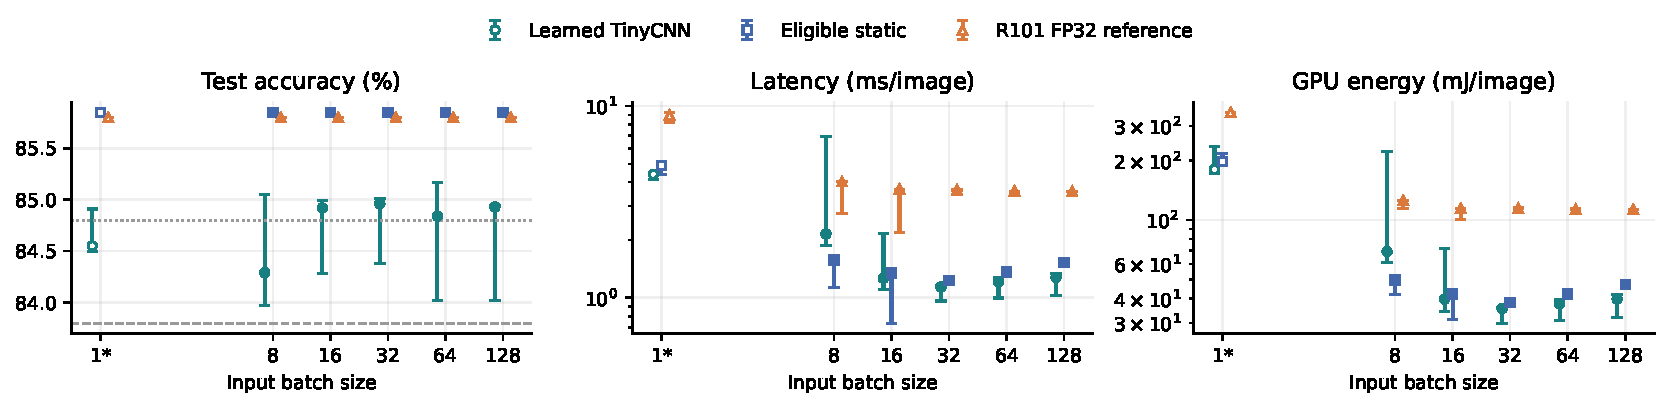
\includegraphics[width=\linewidth]{images/batch_comparison.pdf}\end{center}\vspace{-8 pt}
\smallcap{Teal: learned TinyCNN; blue: eligible static; orange: R101 FP32. Markers: three-seed medians; bars: seed ranges, not confidence intervals. Accuracy lines: 84.80\% (1 pp) and 83.80\% (2 pp). Open batch 1* markers denote Study A's different setup. Costs and baselines are unchanged; startup is separate.}
\begin{center}\small\begin{tabular}{@{}llrrrr@{}}
\toprule
Batch & Protocol & Accuracy (\%) & ms/batch & GPU mJ/batch & Pass\\
\midrule
1 & 6 resident & 84.50--84.91 & 4.15--4.46 & 171.4--235.4 & 1/3\\
8 & 213 choices, cache 2 & 83.97--85.05 & 15.04--55.57 & 485.5--1772.0 & 1/3\\
16 & 213 choices, cache 2 & 84.28--84.99 & 17.58--34.48 & 549.8--1144.0 & 2/3\\
32 & 213 choices, cache 2 & 84.38--85.01 & 30.74--36.88 & 961.3--1151.4 & 2/3\\
64 & 213 choices, cache 2 & 84.02--85.17 & 63.55--80.79 & 1981.5--2511.5 & 2/3\\
128 & 213 choices, cache 2 & 84.02--84.94 & 130.78--169.97 & 4052.9--5306.1 & 2/3\\
\bottomrule
\end{tabular}\end{center}
\smallcap{Batch 1 here is Study A's resident-eager TinyCNN control, not Study B's graph-optimized variant. Table costs average executed batches, including the batch 128 tail (79 batches per 10,000 images). Historical 213 choices/two-engine cache versus new 6 resident candidates are different protocols, not a controlled scaling experiment.}

\textbf{Earlier evidence, retained.} Across all 120 historical settings (both objectives and four allowances), 53 passed accuracy; 31 of these saved latency and 31 saved GPU energy versus their eligible static comparator. The 20 October uniform-random controls reached only 36.26\% accuracy at batch 64 and 36.25\% at 128, versus learned ranges 81.86--85.64\% and 82.25--85.39\%. Beating this weak control does not establish a win over a strong static classifier. Fixed 80\%-pruned controls reached only 0.93--22.55\%: their low costs came with unacceptable accuracy.

\newpage
\heading{2. Batch 1: smaller routers versus runtime optimization}
\textbf{Study A: change the router, keep classifier execution fixed.} Four compact CPU routers and the existing GPU TinyCNN each processed all 10,000 test images for three seeds, once per seed. All six classifiers, execution contexts and buffers stayed loaded in GPU memory, so warm inference had no loading/eviction misses. Standard eager execution was used, without CUDA Graphs.
\begin{center}\small\begin{tabular}{@{}lrrrrrr@{}}
\toprule
Router & Accuracy (\%) & ms/image & GPU mJ/image & Pass 1 pp & Pass 2 pp & Device\\
\midrule
Depth 3 tree & 83.89--85.02 & 4.12--4.98 & 174.5--227.0 & 2/3 & 3/3 & CPU\\
Logistic & 84.01--84.62 & 5.43--5.89 & 221.1--291.3 & 0/3 & 3/3 & CPU\\
Thumbnail MLP & 84.27--84.98 & 4.45--5.16 & 171.6--220.8 & 1/3 & 3/3 & CPU\\
Boosted depth 2 & 84.19--85.01 & 6.59--7.64 & 246.7--305.4 & 1/3 & 3/3 & CPU\\
TinyCNN control & 84.50--84.91 & 4.15--4.46 & 171.4--235.4 & 1/3 & 3/3 & GPU\\
Eligible static & 85.85--85.85 & 4.37--5.10 & 191.6--217.4 & 3/3 & 3/3 & --\\
\bottomrule
\end{tabular}\end{center}
\smallcap{Ranges across three seeds; separate 1 pp/2 pp pass columns assess unchanged runs. Latency is total warm wall time, not router time alone. Four compact alternatives run on CPU, whose energy is excluded from GPU readings. The static model and policies remain validation-selected at 1 pp.}

\textbf{Study A: 1 pp versus 2 pp.} At 1 pp, 5/15 cases pass accuracy and none also saves both latency/GPU energy versus eligible static. At 2 pp, all 15/15 pass accuracy and 4 also show both savings. This is a looser acceptance check on unchanged policies and 1 pp-selected static controls, not a newly optimized 2 pp experiment.


\textbf{Study B: full routing tests of loading/switching changes.} Five variants used the same TinyCNN weights and six classifiers. Three seeds, three repeats, five routed modes and four matched static controls gave 81 full 10,000-image sweeps. These are not isolated microbenchmarks; nor were all changes applied to the compact CPU routers. Compare Study A/B with their own controls, not as a paired speedup.

\textbf{1. Load engine files; keep only two models on GPU.} When the selected model is missing from GPU memory, read its engine file, create its execution context and evict a model if necessary. Selection is dynamic, but repeated switching is expensive. Measured total latency: 15.91--23.15 ms/image; GPU energy: 528.9--806.3 mJ/image.

\textbf{2. Cache engine bytes in CPU RAM and reuse allocations.} Keep verified engine bytes in system RAM to avoid repeated disk reads, reuse buffers and reduce forced cleanup. Only two models are resident on GPU, so misses still require GPU deserialization. The same per-seed choices are preserved. Measured total latency: 7.61--8.20 ms/image; GPU energy: 243.8--285.0 mJ/image.

\textbf{3. Keep all six models on GPU; execute normally.} Load every classifier, its context and buffers before timing. The router can switch among them without warm-run loading or eviction. Eager means ordinary per-inference execution calls, without a captured graph. Measured total latency: 6.66--7.73 ms/image; GPU energy: 197.0--351.6 mJ/image.

\textbf{4. Keep all six models on GPU and replay CUDA Graphs.} In addition to residency, capture GPU work once and replay it to reduce repeated launch overhead. Seed 42 recorded 9.07 \% latency and 4.20 \% GPU-energy savings against graph-enabled eligible static. It meets 1 pp; all three seeds meet 2 pp, but not every repeat improves timing. Measured total latency: 6.07--6.42 ms/image; GPU energy: 190.1--215.3 mJ/image.

\textbf{5. Penalize model switches during selection.} Combine RAM-byte caching with a policy that charges the measured cost of a cache miss. All three seeds then choose R101 FP16 for every image: switching disappears, but selection is constant rather than input-dependent. This is not evidence that dynamic routing beats static selection. Measured total latency: 6.02--6.94 ms/image; GPU energy: 207.4--222.1 mJ/image.


\smallcap{Each cost range spans three seeds' three-repeat medians. Timers include routing, selection, loading/eviction when needed, and classification; startup is separate. Loading, reuse and cleanup changes form a bundle, not an isolated attribution. Static timing varied: lower cost than file loading does not automatically beat a strong static classifier.}

\textbf{Separate engineering probes, not deployed in Studies A/B.}
\begin{itemize}
\item \emph{GPU selection:} compute scores/argmax on GPU and read only the model ID; the CPU still launches a separate classifier engine. Controlled selector timings overlapped (CPU 4.352, Torch GPU 4.368, TensorRT FP32 4.390 ms/image). No reliable speedup; FP32 changed 15/105 near-tie choices.
\item \emph{Native GPU conditional prototype:} two classifiers were combined so only the selected branch ran. It passed branch/parity checks, but took 4.123 ms/image versus 3.955 ms CPU dispatch. This was validation-only engineering, not a full accuracy-qualified routing policy.
\item \emph{Batch 1-specific engine profiles:} a dedicated R34 INT8 build changed 40/100 probe classes (68.06\% validation versus 73.84\% original). It remains quarantined, not counted as an accuracy-preserving optimization. A separate residency probe found 53/12/18 safe models depending on loading order, not an absolute hardware maximum.
\end{itemize}

\newpage
\heading{3. Router-training energy and inference break-even}
\textbf{Measured missing numerator.} Three 20-epoch correctness-router fits were repeated under GPU energy monitoring using seeds 42/45/48. This measures the fitting recipe, not the historical runs retrospectively.
\begin{center}\small
\begin{tabular}{@{}lrrr@{}}\toprule
Router seed & GPU fit energy (J) & Fit-window time (s) & Epochs\\\midrule
42&270.437&11.138&20\\45&201.185&8.389&20\\48&195.008&8.266&20\\\bottomrule
\end{tabular}
\end{center}
Median fit energy is 201.185 J (range 195.008--270.437 J), including initialization, fitting and epoch-checkpoint writes. Supervision, calibration, TensorRT export, final weight writing and CPU/whole-PC energy are excluded. Charge the deployed seed's own fit cost, not all three exploratory fits.

\textbf{Correct denominator: the saving on every inference.} Let $E_{\mathrm{fit}}$ be that router's GPU fitting joules, $e_{\mathrm{static}}$ the comparator's GPU J/image and $e_{\mathrm{route}}$ the \emph{complete routed system's} GPU J/image:
\[
N_{\mathrm{payback}}=\left\lceil\frac{E_{\mathrm{fit}}}{e_{\mathrm{static}}-e_{\mathrm{route}}}\right\rceil .
\]
There is \textbf{no valid payback} when the denominator is nonpositive or held-out accuracy fails. For full batches, the corresponding count is
$\lceil E_{\mathrm{fit}}/[B(e_{\mathrm{static}}-e_{\mathrm{route}})]\rceil$.
This accounts for routing overhead; dividing training energy by static inference energy alone would be incorrect.

\begin{center}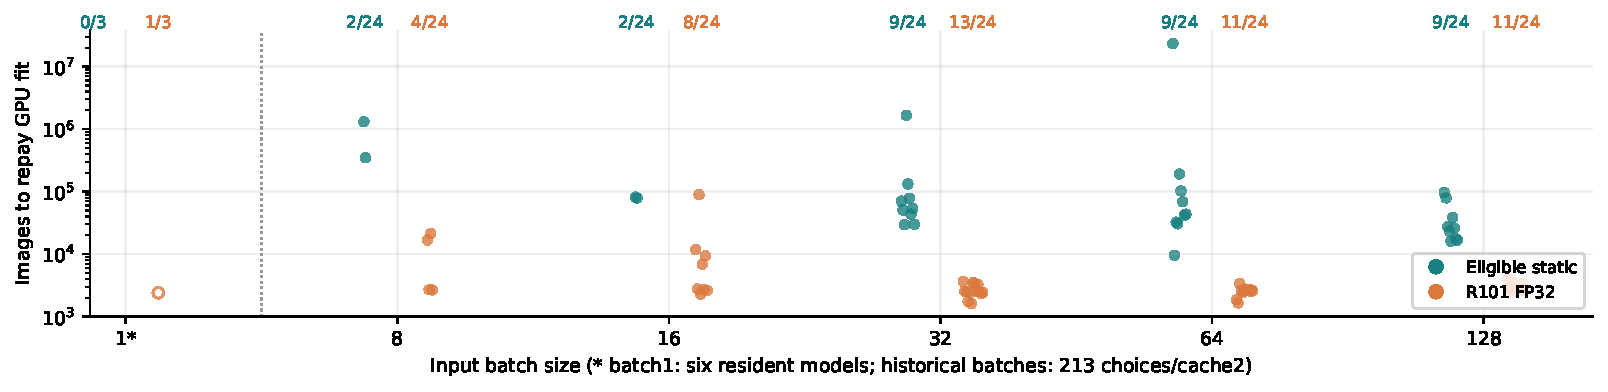
\includegraphics[width=\linewidth]{images/payback_comparison.pdf}\end{center}\vspace{-7 pt}
\smallcap{Batch 1* is Study A's three TinyCNN seeds (latency/1 pp, six resident classifiers, eager), not optimized Study B. Historical batches contain 24 settings each. Each dot is a setting that saves energy and meets its original accuracy allowance. The top count is settings with payback / settings tested. Teal: eligible static; orange: R101 FP32.}
\begin{center}\small\begin{tabular}{@{}rll ll@{}}
\toprule
& \multicolumn{2}{c}{Compared with eligible static} & \multicolumn{2}{c}{Compared with R101 FP32}\\
\cmidrule(lr){2-3}\cmidrule(l){4-5}
Batch & Settings repaying & Images before repayment & Settings repaying & Images before repayment\\
\midrule
1* & No payback & \textemdash & 1 of 3 & 2,399\\
8 & 2 of 24 & 350,497--1,314,076 & 4 of 24 & 2,670--21,288\\
16 & 2 of 24 & 79,015--81,556 & 8 of 24 & 2,279--89,265\\
32 & 9 of 24 & 29,522--1,672,462 & 13 of 24 & 1,614--3,659\\
64 & 9 of 24 & 9,583--23,494,940 & 11 of 24 & 1,653--3,382\\
128 & 9 of 24 & 16,089--96,831 & 11 of 24 & 2,571--3,970\\
\bottomrule
\end{tabular}\end{center}
\textbf{Reading the table.} A \emph{setting} is one seed/objective/allowance combination. ``2 of 24'' means two tested settings repay training energy. ``Images before repayment'' counts images processed by the routed system, not batches; a range spans different settings, not uncertainty. ``No payback'' means no setting both saves energy and meets its original accuracy requirement; the dash means no image count exists.

\textbf{Batch 1 example (Study A, seed 42).} Fitting uses 270.437 J; routed energy is 0.2353969 J/image versus 0.3481643 J/image for R101 FP32: $\lceil 270.437/(0.3481643-0.2353969)\rceil=2,399$ images. Eligible static uses only 0.2173951 J/image, so routing cannot repay energy against it. Other seeds fail the original accuracy gate. CPU-router fit energy is unmeasured, so no CPU-router payback is claimed.


\textbf{Optimized Study B is a different case.} Seed 42 resident-Graph routing uses 0.2153288 GPU J/image and passes accuracy; repayment is 28,621 images versus graph-enabled eligible static. Do not compare this directly with Study A\textquotesingle s 2,399 images versus FP32: the runtime, baseline and measurement session differ.


\textbf{Limits.} These GPU-fit-only estimates combine separate sessions and retain original accuracy requirements, not the new 2 pp sensitivity flags. They exclude CPU/system and preparation energy. Small positive savings yield fragile, very large payback counts; this is not a precise whole-pipeline lifetime-energy account.

\end{document}
